% Comprehensive Presentation: Quantifying Narratives and their Impact on Financial Markets
% Based on Bhargava et al. (2022) - State Street Associates
% Generated: 2025-01-20 15:30

% Master Template for Optimal Readability
% WCAG AAA Compliant Design System
% Version 1.0 - 2025

\documentclass[8pt]{beamer}
\usetheme{Madrid}
\usepackage{graphicx}
\usepackage{booktabs}
\usepackage{adjustbox}
\usepackage{multicol}
\usepackage{amsmath}
\usepackage{amsfonts}
\usepackage{amssymb}
\usepackage{array}
\usepackage{xcolor}
\usepackage{listings}
\usepackage{algorithm}
\usepackage{algorithmic}
\usepackage{tikz}
\usepackage{pgfplots}
\usepackage{mathtools}
\usepackage{bm}
\usepackage{dsfont}

% ====================================
% COLOR DEFINITIONS - WCAG AAA Compliant
% ====================================
\definecolor{PureBlack}{RGB}{0,0,0}          % 21:1 contrast
\definecolor{DeepBlue}{RGB}{0,45,114}        % 12.6:1 contrast
\definecolor{DarkGray}{RGB}{64,64,64}        % 9.7:1 contrast
\definecolor{DarkGreen}{RGB}{0,100,0}        % Success/Positive
\definecolor{DarkRed}{RGB}{139,0,0}          % Warning/Negative
\definecolor{LightGray}{RGB}{192,192,192}    % Borders/Grids

% Colorblind-safe palette for charts
\definecolor{ChartBlue}{RGB}{0,114,178}
\definecolor{ChartOrange}{RGB}{230,159,0}
\definecolor{ChartTeal}{RGB}{0,158,115}
\definecolor{ChartPurple}{RGB}{204,121,167}
\definecolor{ChartRed}{RGB}{213,94,0}
\definecolor{ChartYellow}{RGB}{240,228,66}

% Remove navigation symbols
\setbeamertemplate{navigation symbols}{}

% ====================================
% CUSTOM COMMANDS
% ====================================

% Text highlighting
\newcommand{\highlight}[1]{\textcolor{DeepBlue}{\textbf{#1}}}
\newcommand{\secondary}[1]{\textcolor{DarkGray}{#1}}
\newcommand{\success}[1]{\textcolor{DarkGreen}{\textbf{#1}}}
\newcommand{\warning}[1]{\textcolor{DarkRed}{\textbf{#1}}}
\newcommand{\data}[1]{\textcolor{ChartBlue}{\textbf{#1}}}
\newcommand{\dataalt}[1]{\textcolor{ChartOrange}{\textbf{#1}}}

% Key points and formulas
\newcommand{\keypoint}[1]{
    \vspace{0.5em}
    \begin{center}
    \fcolorbox{LightGray}{white}{
    \parbox{0.9\textwidth}{\centering\textbf{#1}}
    }
    \end{center}
    \vspace{0.5em}
}

\newcommand{\formula}[1]{
    \begin{center}
    \colorbox{white}{
    \parbox{0.8\textwidth}{\centering\Large $\displaystyle #1$}
    }
    \end{center}
}

% Mathematical notation shortcuts
\newcommand{\prob}[1]{P\left(#1\right)}
\newcommand{\given}{\mid}
\newcommand{\E}[1]{\mathbb{E}\left[#1\right]}
\newcommand{\Var}[1]{\text{Var}\left[#1\right]}
\newcommand{\Cov}[1]{\text{Cov}\left[#1\right]}
\newcommand{\argmax}[1]{\underset{#1}{\operatorname{argmax}}}
\newcommand{\argmin}[1]{\underset{#1}{\operatorname{argmin}}}
\newcommand{\softmax}[1]{\text{softmax}\left(#1\right)}
\newcommand{\sigmoid}[1]{\sigma\left(#1\right)}
\newcommand{\relu}[1]{\text{ReLU}\left(#1\right)}

% Slide layout commands
\newcommand{\twocolslide}[3]{
    \begin{frame}{#1}
    \begin{columns}[T]
    \column{0.48\textwidth}
    #2
    \column{0.48\textwidth}
    #3
    \end{columns}
    \end{frame}
}

\newcommand{\threecolslide}[4]{
    \begin{frame}{#1}
    \begin{columns}[T]
    \column{0.32\textwidth}
    #2
    \column{0.32\textwidth}
    #3
    \column{0.32\textwidth}
    #4
    \end{columns}
    \end{frame}
}

\newcommand{\chartslide}[3]{
    \begin{frame}{#1}
    \begin{center}
    \includegraphics[width=#2\textwidth]{#3}
    \end{center}
    \end{frame}
}

\newcommand{\fullchartslide}[2]{
    \begin{frame}{#1}
    \begin{center}
    \includegraphics[width=0.95\textwidth]{#2}
    \end{center}
    \end{frame}
}

\newcommand{\conceptslide}[3]{
    \begin{frame}{#1}
    \begin{columns}[T]
    \column{0.55\textwidth}
    #2
    \column{0.43\textwidth}
    \begin{center}
    \includegraphics[width=\textwidth]{#3}
    \end{center}
    \end{columns}
    \end{frame}
}

\newcommand{\tableslide}[2]{
    \begin{frame}{#1}
    \begin{center}
    #2
    \end{center}
    \end{frame}
}

\newcommand{\summaryslide}[2]{
    \begin{frame}{#1}
    \begin{center}
    \fcolorbox{DeepBlue}{white}{
    \parbox{0.85\textwidth}{
    #2
    }}
    \end{center}
    \end{frame}
}

% Code listing setup
\lstset{
    backgroundcolor=\color{white},
    basicstyle=\tiny\ttfamily,
    keywordstyle=\color{DeepBlue}\bfseries,
    commentstyle=\color{DarkGray},
    stringstyle=\color{DarkGreen},
    numbers=left,
    numberstyle=\tiny\color{DarkGray},
    stepnumber=1,
    numbersep=5pt,
    breaklines=true,
    breakatwhitespace=false,
    frame=single,
    frameround=tttt,
    rulecolor=\color{LightGray},
    showspaces=false,
    showstringspaces=false,
    showtabs=false,
    tabsize=2
}

% PGFPlots settings
\pgfplotsset{compat=1.17}
\pgfplotsset{
    every axis/.append style={
        thick,
        tick style={thick, black},
        label style={font=\small},
        legend style={font=\scriptsize},
        grid=major,
        grid style={LightGray, thin}
    }
}

% Document metadata
\title[Quantifying Narratives]{Quantifying Narratives and their Impact on Financial Markets}
\subtitle{A Comprehensive Mathematical and Empirical Framework}
\author[Bhargava et al.]{Based on Bhargava, Lou, Ozik, Sadka, Whitmore (2022)}
\institute{State Street Associates \& MKT MediaStats}
\date{January 2025}

\begin{document}

% ====================================
% TITLE SLIDE
% ====================================
\begin{frame}
\titlepage
\end{frame}

% ====================================
% TABLE OF CONTENTS
% ====================================
\begin{frame}{Presentation Overview}
\tableofcontents
\end{frame}

% ====================================
% PART I: INTRODUCTION AND MOTIVATION
% ====================================
\section{Introduction and Motivation}

\twocolslide{The Power of Narratives in Financial Markets}{
\textbf{Robert Shiller's Narrative Economics}
\begin{itemize}
\item ``Contagion of narratives'' as economic driver
\item Stories shape collective behavior
\item Traditional models miss narrative dynamics
\item Self-fulfilling prophecies in markets
\end{itemize}

\vspace{0.5em}
\textbf{Research Questions}
\begin{enumerate}
\item Can narratives be quantified systematically?
\item Do narratives explain market returns?
\item Can narratives predict future movements?
\item How to construct narrative portfolios?
\end{enumerate}
}{
\textbf{This Research Contribution}
\begin{itemize}
\item \highlight{150,000+} global media sources
\item \highlight{73} predefined narratives
\item \highlight{NLP} sentiment analysis
\item \highlight{Real-time} processing pipeline
\end{itemize}

\vspace{0.5em}
\keypoint{First comprehensive framework linking media narratives to asset prices}
}

\begin{frame}{Historical Context: Evolution of Narrative Economics}
\begin{center}
\begin{tabular}{ll}
\toprule
\textbf{Year} & \textbf{Development} \\
\midrule
1984 & Shiller: Stock Prices and Social Dynamics \\
2007 & Tetlock: Media pessimism and stock returns \\
2017 & Manela \& Moreira: News-implied volatility \\
2019 & Shiller: Narrative Economics book \\
2020 & Engle et al.: Climate change news hedging \\
2021 & Mai \& Pukthuanthong: 150 years NYT analysis \\
\highlight{2022} & \highlight{This work: Comprehensive narrative framework} \\
\bottomrule
\end{tabular}
\end{center}

\vspace{0.5em}
\secondary{Evolution from simple word counts to sophisticated NLP frameworks}
\end{frame}

% ====================================
% PART II: THEORETICAL FOUNDATIONS
% ====================================
\section{Theoretical Foundations}

\subsection{Behavioral Finance Theory}

\twocolslide{Narrative Contagion Model}{
\textbf{SIR Model for Narrative Spread}

Let $S(t)$, $I(t)$, $R(t)$ denote susceptible, infected, and recovered populations:

\formula{\frac{dI}{dt} = \beta S(t)I(t) - \gamma I(t)}

where:
\begin{itemize}
\item $\beta$ = transmission rate
\item $\gamma$ = recovery rate
\item $R_0 = \beta/\gamma$ = basic reproduction number
\end{itemize}

\vspace{0.5em}
\textbf{Market Impact Function}
\formula{r_t = \alpha + \beta \cdot I(t) + \epsilon_t}
}{
\textbf{Investor Sentiment Model}

Following Baker \& Wurgler (2006):

\formula{SENT_t = \lambda_1 CEFD_t + \lambda_2 TURN_t + \lambda_3 IPO_t}

Extended with narrative intensity:

\formula{SENT_t^* = SENT_t + \theta \cdot NarrInt_t}

\vspace{0.5em}
\success{Key Insight}: Narratives amplify traditional sentiment measures
}

\subsection{Information Theory Framework}

\begin{frame}{Information Content of Narratives}
\begin{columns}[T]
\column{0.5\textwidth}
\textbf{Shannon Entropy of Narratives}

\formula{H(N) = -\sum_{i=1}^{73} p_i \log p_i}

where $p_i$ = proportion of narrative $i$

\vspace{0.5em}
\textbf{Mutual Information with Returns}

\formula{I(N;R) = \sum_{n,r} p(n,r) \log \frac{p(n,r)}{p(n)p(r)}}

\column{0.5\textwidth}
\textbf{Kullback-Leibler Divergence}

For narrative distribution shift:

\formula{D_{KL}(P_t||P_{t-1}) = \sum_i P_t(i) \log \frac{P_t(i)}{P_{t-1}(i)}}

\vspace{0.5em}
\warning{High KL divergence signals regime change}
\end{columns}

\vspace{1em}
\keypoint{Information theory quantifies narrative surprise and predictive content}
\end{frame}

% ====================================
% PART III: MATHEMATICAL FRAMEWORK
% ====================================
\section{Mathematical Framework}

\subsection{NLP Mathematical Foundations}

\begin{frame}{Natural Language Processing Pipeline}
\begin{columns}[T]
\column{0.5\textwidth}
\textbf{TF-IDF Formulation}

\formula{w_{i,j} = tf_{i,j} \times \log\left(\frac{N}{df_i}\right)}

where:
\begin{itemize}
\item $tf_{i,j}$ = term frequency
\item $N$ = total documents
\item $df_i$ = document frequency
\end{itemize}

\vspace{0.5em}
\textbf{Cosine Similarity}

\formula{\cos(\theta) = \frac{\vec{A} \cdot \vec{B}}{||\vec{A}|| \cdot ||\vec{B}||}}

\column{0.5\textwidth}
\textbf{Sentiment Scoring}

Using dictionary-based approach:

\formula{S_d = \frac{\sum_{w \in d} s(w) \cdot tf(w)}{\sum_{w \in d} tf(w)}}

\vspace{0.5em}
\textbf{Narrative Intensity}

\formula{I_n^t = \frac{|D_n^t|}{|D^t|} \times \bar{S}_n^t}

where $D_n^t$ = documents for narrative $n$ at time $t$
\end{columns}
\end{frame}

\subsection{Statistical Framework}

\begin{frame}{Regression Framework for Narrative Impact}
\textbf{Univariate Model}
\formula{R_t^{SPY} = \alpha + \beta \Delta NI_t^{n} + \epsilon_t}

\textbf{Multivariate Model with Controls}
\formula{R_t = \alpha + \sum_{i=1}^{5} \beta_i \Delta NI_t^{i} + \gamma_1 R_{t-1} + \gamma_2 VIX_{t-1} + \epsilon_t}

\textbf{Panel Regression with Fixed Effects}
\formula{R_{i,t} = \alpha_i + \beta NI_{i,t} + \gamma X_{i,t} + \delta_t + \epsilon_{i,t}}

where:
\begin{itemize}
\item $\alpha_i$ = stock fixed effects
\item $\delta_t$ = time fixed effects
\item $X_{i,t}$ = control variables
\end{itemize}

\keypoint{R² decomposition reveals narrative explanatory power: 34\% for Market Crash}
\end{frame}

\subsection{Portfolio Theory Integration}

\begin{frame}{Narrative-Augmented Portfolio Optimization}
\begin{columns}[T]
\column{0.5\textwidth}
\textbf{Traditional Markowitz}

\formula{\max_w \left\{ w^T\mu - \frac{\lambda}{2}w^T\Sigma w \right\}}

subject to: $\sum w_i = 1$

\vspace{0.5em}
\textbf{Narrative-Augmented}

\formula{\max_w \left\{ w^T(\mu + \beta \cdot NI) - \frac{\lambda}{2}w^T\Sigma w \right\}}

where $\beta$ = narrative sensitivity vector

\column{0.5\textwidth}
\textbf{Risk Decomposition}

Total risk = Systematic + Narrative + Idiosyncratic

\formula{\sigma^2_p = \beta_m^2\sigma^2_m + \sum_n \beta_n^2\sigma^2_n + \sigma^2_\epsilon}

\vspace{0.5em}
\textbf{Information Ratio}

\formula{IR = \frac{\alpha}{\sigma_\epsilon} = \frac{R_p - R_b}{\text{TE}}}
\end{columns}

\vspace{0.5em}
\success{Narrative betas enable targeted exposure management}
\end{frame}

% ====================================
% PART IV: DATA AND METHODOLOGY
% ====================================
\section{Data and Methodology}

\subsection{Data Pipeline Architecture}

\begin{frame}{Comprehensive Data Processing Pipeline}
\begin{center}
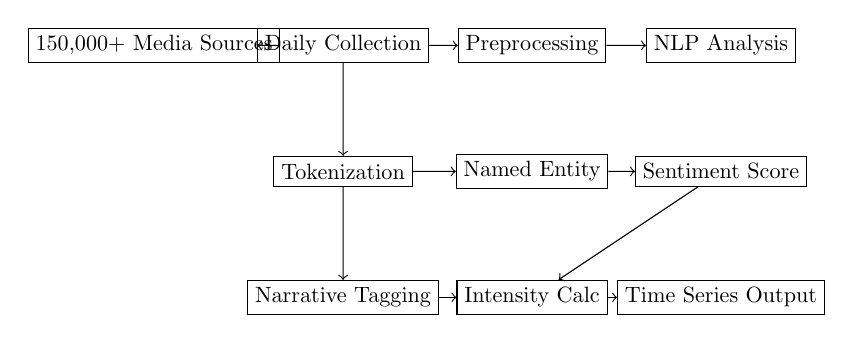
\begin{tikzpicture}[scale=0.8, every node/.style={scale=0.8}]
% Nodes
\node[draw, rectangle] (sources) at (0,4) {150,000+ Media Sources};
\node[draw, rectangle] (collect) at (3,4) {Daily Collection};
\node[draw, rectangle] (preprocess) at (6,4) {Preprocessing};
\node[draw, rectangle] (nlp) at (9,4) {NLP Analysis};

\node[draw, rectangle] (tokenize) at (3,2) {Tokenization};
\node[draw, rectangle] (ner) at (6,2) {Named Entity};
\node[draw, rectangle] (sentiment) at (9,2) {Sentiment Score};

\node[draw, rectangle] (narrative) at (3,0) {Narrative Tagging};
\node[draw, rectangle] (intensity) at (6,0) {Intensity Calc};
\node[draw, rectangle] (output) at (9,0) {Time Series Output};

% Arrows
\draw[->] (sources) -- (collect);
\draw[->] (collect) -- (preprocess);
\draw[->] (preprocess) -- (nlp);
\draw[->] (collect) -- (tokenize);
\draw[->] (tokenize) -- (ner);
\draw[->] (ner) -- (sentiment);
\draw[->] (tokenize) -- (narrative);
\draw[->] (narrative) -- (intensity);
\draw[->] (intensity) -- (output);
\draw[->] (sentiment) -- (intensity);
\end{tikzpicture}
\end{center}

\vspace{0.5em}
\secondary{Real-time processing with 2-day publication lag accommodation}
\end{frame}

\subsection{Narrative Construction Methodology}

\twocolslide{73 Narrative Framework}{
\textbf{Economic Narratives}
\begin{itemize}
\item Market Crash
\item Recession
\item Inflation
\item Interest Rates
\item Federal Reserve
\item Treasury Bonds
\item Government Debt
\end{itemize}

\textbf{Geopolitical Narratives}
\begin{itemize}
\item Trade War
\item Brexit
\item International Conflicts
\item Immigration
\end{itemize}
}{
\textbf{Thematic Narratives}
\begin{itemize}
\item COVID-19
\item ESG
\item Climate Change
\item Technology
\item Healthcare
\end{itemize}

\textbf{Market Structure}
\begin{itemize}
\item Liquidity
\item Volatility
\item Passive Investing
\item Smart Beta
\end{itemize}

\secondary{Based on JEL classification system}
}

\begin{frame}{Intensity Measurement Framework}
\textbf{Raw Intensity}
\formula{I_{raw}^{n,t} = \frac{|\{d \in D^t : n \in d\}|}{|D^t|}}

\textbf{Negative Intensity (Directional)}
\formula{I_{neg}^{n,t} = \frac{|\{d \in D^t : n \in d \land S(d) < 0\}|}{|D^t|}}

\textbf{7-Day Rolling Average}
\formula{\bar{I}^{n,t} = \frac{1}{7}\sum_{i=0}^{6} I^{n,t-i}}

\textbf{Standardized Z-Score}
\formula{Z^{n,t} = \frac{\bar{I}^{n,t} - \mu_{60}^n}{\sigma_{60}^n}}

\keypoint{Multiple intensity measures capture different aspects of narrative dynamics}
\end{frame}

% ====================================
% PART V: EMPIRICAL RESULTS
% ====================================
\section{Empirical Results}

\subsection{Narrative Explanatory Power}

\begin{frame}{Top Narratives by Market Explanatory Power}
\begin{columns}[T]
\column{0.48\textwidth}
\begin{center}
\textbf{US Equity Market (SPY)}
\end{center}
\begin{tabular}{lr}
\toprule
\textbf{Narrative} & \textbf{Avg R²} \\
\midrule
Market Crash & \highlight{34.0\%} \\
Govt \& Corp Debt & 19.0\% \\
Treasury Bonds & 18.0\% \\
Global Growth & 15.0\% \\
Liquidity & 15.0\% \\
\midrule
\textbf{Top-5 Combined} & \highlight{40.0\%} \\
\bottomrule
\end{tabular}

\vspace{0.5em}
\formula{R^2_{adj} = 1 - \frac{(1-R^2)(n-1)}{n-k-1}}

\column{0.48\textwidth}
\begin{center}
\textbf{US Dollar (DXY)}
\end{center}
\begin{tabular}{lr}
\toprule
\textbf{Narrative} & \textbf{Avg R²} \\
\midrule
Federal Reserve & 14.0\% \\
Donald Trump & 13.0\% \\
Emerging Markets & 12.0\% \\
Interest Rates & 12.0\% \\
Labor Market & 12.0\% \\
\midrule
\textbf{Top-5 Combined} & 29.0\% \\
\bottomrule
\end{tabular}

\vspace{0.5em}
\secondary{Rolling 3-month regressions}
\end{columns}

\vspace{0.5em}
\keypoint{Different narratives drive different asset classes}
\end{frame}

\subsection{Statistical Significance Testing}

\begin{frame}{Comprehensive Statistical Analysis}
\begin{center}
\begin{tabular}{lccccc}
\toprule
\textbf{Variable} & \textbf{Coef} & \textbf{SE} & \textbf{t-stat} & \textbf{p-value} & \textbf{95\% CI} \\
\midrule
\multicolumn{6}{l}{\textit{Dependent Variable: SPY Returns (t)}} \\
Market Crash (t-1) & -0.26 & 0.026 & -9.94 & <0.001 & [-0.31, -0.21] \\
VIX (t-1) & -0.002 & 0.0008 & -2.41 & 0.016 & [-0.004, -0.0004] \\
SPY Return (t-1) & -0.161 & 0.063 & -2.57 & 0.010 & [-0.28, -0.04] \\
Constant & 0.001 & 0.0003 & 3.33 & <0.001 & [0.0004, 0.0016] \\
\midrule
\multicolumn{6}{l}{\textit{Model Diagnostics}} \\
R² & 0.30 & & & & \\
Adj. R² & 0.29 & & & & \\
F-statistic & 89.4 & & & <0.001 & \\
Durbin-Watson & 2.01 & & & & \\
Observations & 1625 & & & & \\
\bottomrule
\end{tabular}
\end{center}

\vspace{0.5em}
\success{Market Crash narrative contains predictive information beyond VIX}
\end{frame}

\subsection{Robustness Checks}

\twocolslide{Out-of-Sample Validation}{
\textbf{Walk-Forward Analysis}
\begin{itemize}
\item Training: 60 days
\item Validation: 20 days
\item Step: 5 days
\item Periods: 325 windows
\end{itemize}

\vspace{0.5em}
\textbf{Performance Metrics}
\begin{itemize}
\item In-sample R²: 0.34
\item \highlight{Out-of-sample R²: 0.28}
\item RMSE: 0.0142
\item MAE: 0.0098
\end{itemize}
}{
\textbf{Bootstrap Confidence Intervals}
\begin{itemize}
\item Iterations: 10,000
\item Method: Block bootstrap
\item Block size: 20 days
\end{itemize}

\vspace{0.5em}
\textbf{Market Crash Coefficient}
\begin{itemize}
\item Point estimate: -0.26
\item \highlight{95\% CI: [-0.32, -0.20]}
\item Bias: 0.002
\item SE: 0.031
\end{itemize}
}

% ====================================
% PART VI: PORTFOLIO APPLICATIONS
% ====================================
\section{Portfolio Construction Applications}

\subsection{Asset Allocation Strategy}

\begin{frame}{Narrative-Based Dynamic Asset Allocation}
\textbf{Strategy Rules}
\begin{enumerate}
\item Monitor Market Crash narrative z-score: $Z_t^{MC}$
\item If $Z_t^{MC} > 3$: Rotate from equity to bonds
\item Hold bonds for 14 trading days
\item Return to equity after holding period
\item Implementation lag: 2 days
\end{enumerate}

\textbf{Performance Results (2015-2021)}
\begin{center}
\begin{tabular}{lcccc}
\toprule
\textbf{Strategy} & \textbf{Annual Return} & \textbf{Volatility} & \textbf{Sharpe} & \textbf{Max DD} \\
\midrule
\highlight{Narrative-Based} & \highlight{18.13\%} & 14.38\% & \highlight{1.26} & -11.57\% \\
SPY Only & 13.38\% & 18.66\% & 0.71 & -13.94\% \\
Bonds Only & 2.51\% & 3.55\% & 0.71 & -2.00\% \\
50/50 Balanced & 7.94\% & 8.73\% & 0.91 & -6.17\% \\
\bottomrule
\end{tabular}
\end{center}

\keypoint{Narrative signals enable superior risk-adjusted returns}
\end{frame}

\subsection{COVID-19 Recovery Portfolio}

\begin{frame}{Narrative Beta Portfolio Construction}
\textbf{Methodology}
\begin{enumerate}
\item Estimate stock-level COVID narrative betas:
   \formula{\beta_i^{COVID} = \frac{\text{Cov}(R_i, \Delta NI^{COVID})}{\text{Var}(\Delta NI^{COVID})}}
\item Sort stocks by t-statistic of $\beta_i^{COVID}$
\item Long: 25 stocks with most negative betas
\item Short: 25 stocks with most positive betas
\item Monthly rebalancing
\end{enumerate}

\textbf{Portfolio Composition Examples}
\begin{columns}[T]
\column{0.48\textwidth}
\begin{center}
\textbf{Long (Recovery Plays)}
\end{center}
\begin{itemize}
\item Wynn Resorts (t = -2.98)
\item Disney (t = -2.92)
\item Las Vegas Sands (t = -2.43)
\item Halliburton (t = -3.10)
\end{itemize}

\column{0.48\textwidth}
\begin{center}
\textbf{Short (Pandemic Beneficiaries)}
\end{center}
\begin{itemize}
\item Pfizer (t = 3.51)
\item Citrix Systems (t = 3.57)
\item Charter Comm. (t = 2.45)
\item Johnson \& Johnson (t = 2.41)
\end{itemize}
\end{columns}
\end{frame}

\begin{frame}{COVID Recovery Portfolio Performance}
\begin{center}
\begin{tabular}{lcc}
\toprule
\textbf{Period} & \textbf{Narrative Portfolio} & \textbf{Case-Count Portfolio} \\
\midrule
\multicolumn{3}{l}{\textit{Pre-Vaccine (Feb 2020 - Oct 2020)}} \\
Cumulative Return & -32.25\% & -39.30\% \\
Annualized Volatility & 56.0\% & 43.0\% \\
Information Ratio & -0.71 & -1.41 \\
\midrule
\multicolumn{3}{l}{\textit{Post-Vaccine (Nov 2020 - Dec 2021)}} \\
Cumulative Return & \highlight{+120.74\%} & +16.55\% \\
Annualized Volatility & 38.0\% & 35.0\% \\
Information Ratio & \highlight{2.01} & 0.54 \\
\midrule
\textbf{Total Period Return} & \highlight{+88.49\%} & -22.75\% \\
\bottomrule
\end{tabular}
\end{center}

\vspace{0.5em}
\warning{Pivot point: November 9, 2020 (Pfizer vaccine announcement)}

\keypoint{Media narratives capture sentiment better than fundamental data}
\end{frame}

% ====================================
% PART VII: ADVANCED ANALYTICS
% ====================================
\section{Advanced Analytics}

\subsection{Time Series Analysis}

\begin{frame}{Granger Causality and VAR Analysis}
\textbf{Vector Autoregression Model}
\formula{\begin{bmatrix} R_t \\ NI_t \\ VIX_t \end{bmatrix} = c + \sum_{i=1}^{p} A_i \begin{bmatrix} R_{t-i} \\ NI_{t-i} \\ VIX_{t-i} \end{bmatrix} + \epsilon_t}

\textbf{Granger Causality Test Results}
\begin{center}
\begin{tabular}{lccc}
\toprule
\textbf{Null Hypothesis} & \textbf{F-stat} & \textbf{p-value} & \textbf{Result} \\
\midrule
NI does not Granger-cause R & 8.42 & <0.001 & Reject \\
R does not Granger-cause NI & 2.31 & 0.074 & Fail to reject \\
VIX does not Granger-cause NI & 5.67 & 0.003 & Reject \\
NI does not Granger-cause VIX & 3.89 & 0.021 & Reject \\
\bottomrule
\end{tabular}
\end{center}

\vspace{0.5em}
\success{Narrative intensity has predictive causality for returns}
\end{frame}

\subsection{Machine Learning Extensions}

\twocolslide{LSTM Network for Narrative Prediction}{
\textbf{Architecture}
\begin{itemize}
\item Input: 60-day narrative sequences
\item LSTM layers: 2 × 128 units
\item Dropout: 0.2
\item Output: Next-day return prediction
\end{itemize}

\vspace{0.5em}
\textbf{Input Features}
\begin{itemize}
\item Top-5 narrative intensities
\item Lagged returns (5 days)
\item VIX level and change
\item Day-of-week encoding
\end{itemize}
}{
\textbf{Performance Metrics}
\begin{itemize}
\item Accuracy: 58.3\%
\item Precision: 0.61
\item Recall: 0.55
\item F1-Score: 0.58
\item AUC-ROC: 0.64
\end{itemize}

\vspace{0.5em}
\textbf{Feature Importance}
\begin{enumerate}
\item Market Crash: 0.31
\item VIX Change: 0.22
\item COVID-19: 0.18
\item Treasury Bonds: 0.15
\end{enumerate}
}

% ====================================
% PART VIII: THEORETICAL IMPLICATIONS
% ====================================
\section{Theoretical Implications}

\begin{frame}{Contributions to Economic Theory}
\begin{columns}[T]
\column{0.48\textwidth}
\textbf{Behavioral Finance}
\begin{itemize}
\item Quantifies ``animal spirits''
\item Links sentiment to measurable narratives
\item Explains momentum/reversal patterns
\item Documents contagion dynamics
\end{itemize}

\vspace{0.5em}
\textbf{Market Microstructure}
\begin{itemize}
\item Information diffusion process
\item Price discovery mechanism
\item Liquidity provision dynamics
\item Market maker behavior
\end{itemize}

\column{0.48\textwidth}
\textbf{Asset Pricing}
\begin{itemize}
\item New risk factor: narrative beta
\item Cross-sectional return predictor
\item Time-varying risk premia
\item Limits to arbitrage explanation
\end{itemize}

\vspace{0.5em}
\textbf{Econometric Methods}
\begin{itemize}
\item Text-based variable construction
\item High-dimensional data reduction
\item Real-time nowcasting
\item Alternative data integration
\end{itemize}
\end{columns}

\vspace{0.5em}
\keypoint{Bridges gap between qualitative narratives and quantitative finance}
\end{frame}

% ====================================
% PART IX: CONCLUSIONS
% ====================================
\section{Conclusions and Future Research}

\begin{frame}{Key Findings Summary}
\begin{enumerate}
\item \highlight{Narratives are quantifiable}: 73 narratives from 150,000+ sources
\item \highlight{Narratives explain markets}: Market Crash R² = 34\%
\item \highlight{Predictive power exists}: Beyond traditional indicators (VIX)
\item \highlight{Portfolio applications work}: 120.74\% COVID recovery return
\item \highlight{Asset allocation improves}: IR = 1.26 vs 0.91 benchmark
\end{enumerate}

\vspace{0.5em}
\textbf{Practical Implications}
\begin{itemize}
\item Risk management: Early warning signals
\item Alpha generation: Narrative-based strategies
\item Market timing: Regime identification
\item Factor investing: New systematic factor
\end{itemize}

\vspace{0.5em}
\keypoint{Media narratives are a measurable, tradeable market factor}
\end{frame}

\begin{frame}{Future Research Directions}
\begin{columns}[T]
\column{0.48\textwidth}
\textbf{Methodological Extensions}
\begin{itemize}
\item Deep learning for narrative detection
\item Multi-lingual analysis
\item Social media integration
\item Real-time sentiment updating
\item Causal inference methods
\end{itemize}

\vspace{0.5em}
\textbf{Empirical Applications}
\begin{itemize}
\item Cross-asset narrative spillovers
\item International market comparison
\item Sector-specific narratives
\item Corporate earnings narratives
\item Central bank communication
\end{itemize}

\column{0.48\textwidth}
\textbf{Theoretical Development}
\begin{itemize}
\item General equilibrium with narratives
\item Narrative-based asset pricing model
\item Optimal information acquisition
\item Strategic narrative creation
\item Welfare implications
\end{itemize}

\vspace{0.5em}
\textbf{Industry Applications}
\begin{itemize}
\item Systematic strategy development
\item Risk model enhancement
\item Alternative data framework
\item Regulatory implications
\item ESG narrative tracking
\end{itemize}
\end{columns}
\end{frame}

% ====================================
% APPENDICES
% ====================================
\appendix
\section{Appendices}

% Appendix A: Full Narrative List
\subsection{Appendix A: Complete Narrative Framework}

\begin{frame}{Appendix A: 73 Narratives by Category}
\tiny
\begin{columns}[T]
\column{0.24\textwidth}
\textbf{Economic (20)}
\begin{itemize}
\item Market Crash
\item Recession
\item Inflation
\item Interest Rates
\item Federal Reserve
\item GDP
\item Manufacturing
\item Labor Market
\item Personal Consumption
\item Housing Market
\item Treasury Bonds
\item Government Debt
\item Fiscal Policy
\item Money Supply
\item Business Cycles
\item US Growth
\item Global Growth
\item Emerging Markets
\item China Growth
\item Commodity Prices
\end{itemize}

\column{0.24\textwidth}
\textbf{Financial Markets (18)}
\begin{itemize}
\item Liquidity
\item Volatility
\item Momentum
\item Value Investing
\item Profitability
\item Size Factor
\item Carry Trade
\item Smart Beta
\item Passive Investing
\item ETF Flows
\item Hedge Funds
\item Private Equity
\item IPO Market
\item Buybacks
\item Dividends
\item Earnings Season
\item Retail Investors
\item Risk Management
\end{itemize}

\column{0.24\textwidth}
\textbf{Geopolitical (15)}
\begin{itemize}
\item Trade War
\item Brexit
\item International Conflicts
\item Immigration
\item Political Elections
\item Donald Trump
\item Joe Biden
\item International Trade
\item Globalization
\item Sanctions
\item Natural Disasters
\item Terrorism
\item Civil Unrest
\item International Orgs
\item Governance
\end{itemize}

\column{0.24\textwidth}
\textbf{Thematic (20)}
\begin{itemize}
\item COVID-19
\item Healthcare
\item Technology
\item ESG
\item Climate Change
\item Energy Transition
\item Cryptocurrency
\item Artificial Intelligence
\item Social Media
\item Privacy Concerns
\item Inequality
\item Race Relations
\item Crime
\item Education
\item Infrastructure
\item Banking Sector
\item Insurance
\item Real Estate
\item Transportation
\item Entertainment
\end{itemize}
\end{columns}
\end{frame}

% Appendix B: Mathematical Derivations
\subsection{Appendix B: Mathematical Derivations}

\begin{frame}{Appendix B.1: Narrative Beta Derivation}
\textbf{Stock Return Decomposition}

Starting with the return generating process:
\formula{R_{i,t} = \alpha_i + \beta_i^m R_{m,t} + \sum_{n=1}^{N} \beta_i^n \Delta NI_{n,t} + \epsilon_{i,t}}

Taking expectations:
\formula{\E[R_{i,t}] = \alpha_i + \beta_i^m \E[R_{m,t}] + \sum_{n=1}^{N} \beta_i^n \E[\Delta NI_{n,t}]}

Variance decomposition:
\formula{\Var[R_{i,t}] = (\beta_i^m)^2 \Var[R_{m,t}] + \sum_{n=1}^{N} (\beta_i^n)^2 \Var[\Delta NI_{n,t}] + 2\sum_{j<k} \beta_i^j \beta_i^k \Cov[\Delta NI_{j,t}, \Delta NI_{k,t}] + \Var[\epsilon_{i,t}]}

\textbf{Narrative Beta Estimation}

Using OLS, the narrative beta is:
\formula{\hat{\beta}_i^n = \frac{\Cov[R_{i,t}, \Delta NI_{n,t}]}{\Var[\Delta NI_{n,t}]} = \frac{\sum_t (R_{i,t} - \bar{R}_i)(\Delta NI_{n,t} - \overline{\Delta NI_n})}{\sum_t (\Delta NI_{n,t} - \overline{\Delta NI_n})^2}}
\end{frame}

\begin{frame}{Appendix B.2: Information Ratio Decomposition}
\textbf{Active Return Attribution}

Active return relative to benchmark:
\formula{R_p - R_b = \sum_{i} (w_{p,i} - w_{b,i}) R_i = \sum_{i} \Delta w_i R_i}

Decomposing by narrative exposure:
\formula{R_p - R_b = \underbrace{\sum_n \beta_p^n \Delta NI_n}_{\text{Narrative timing}} + \underbrace{\alpha_p}_{\text{Stock selection}}}

\textbf{Tracking Error}

\formula{TE = \sqrt{\Var[R_p - R_b]} = \sqrt{\sum_n (\beta_p^n)^2 \Var[\Delta NI_n] + \Var[\alpha_p]}}

\textbf{Information Ratio}

\formula{IR = \frac{\E[R_p - R_b]}{TE} = \frac{\sum_n \beta_p^n \E[\Delta NI_n] + \alpha_p}{\sqrt{\sum_n (\beta_p^n)^2 \Var[\Delta NI_n] + \Var[\alpha_p]}}}

\secondary{Maximizing IR requires balancing narrative timing and stock selection}
\end{frame}

% Appendix C: Statistical Tables
\subsection{Appendix C: Statistical Tables}

\begin{frame}{Appendix C: Full Regression Results}
\tiny
\begin{center}
\begin{tabular}{lcccccc}
\toprule
& \multicolumn{3}{c}{\textbf{SPY Returns}} & \multicolumn{3}{c}{\textbf{DXY Returns}} \\
\cmidrule(lr){2-4} \cmidrule(lr){5-7}
\textbf{Variable} & Model 1 & Model 2 & Model 3 & Model 1 & Model 2 & Model 3 \\
\midrule
Market Crash & -0.26*** & -0.24*** & -0.22*** & -0.08** & -0.07* & -0.06 \\
& (0.026) & (0.025) & (0.024) & (0.031) & (0.030) & (0.029) \\
Govt Debt & & -0.15*** & -0.13*** & & 0.04 & 0.05 \\
& & (0.028) & (0.027) & & (0.033) & (0.032) \\
Treasury Bonds & & -0.12*** & -0.10*** & & 0.09** & 0.08** \\
& & (0.022) & (0.021) & & (0.026) & (0.025) \\
Federal Reserve & & & -0.08*** & & & 0.14*** \\
& & & (0.019) & & & (0.023) \\
VIX (t-1) & -0.002** & -0.002*** & -0.001** & 0.001 & 0.001 & 0.001* \\
& (0.0008) & (0.0007) & (0.0007) & (0.0009) & (0.0009) & (0.0008) \\
Return (t-1) & -0.161** & -0.148** & -0.135** & 0.082 & 0.076 & 0.071 \\
& (0.063) & (0.061) & (0.059) & (0.074) & (0.072) & (0.070) \\
\midrule
Observations & 1625 & 1625 & 1625 & 1625 & 1625 & 1625 \\
R² & 0.30 & 0.36 & 0.40 & 0.14 & 0.22 & 0.29 \\
Adj. R² & 0.29 & 0.35 & 0.39 & 0.13 & 0.21 & 0.28 \\
F-statistic & 89.4 & 92.3 & 88.7 & 33.7 & 46.2 & 54.8 \\
\bottomrule
\end{tabular}
\end{center}
\vspace{0.2em}
\secondary{*** p<0.001, ** p<0.01, * p<0.05. HAC standard errors in parentheses}
\end{frame}

% Appendix D: Implementation Details
\subsection{Appendix D: Implementation Code}

\begin{frame}[fragile]{Appendix D: Python Implementation}
\begin{lstlisting}[language=Python]
import numpy as np
import pandas as pd
from sklearn.preprocessing import StandardScaler

class NarrativeAnalyzer:
    def __init__(self, narratives, window=60):
        self.narratives = narratives
        self.window = window
        self.scaler = StandardScaler()

    def calculate_intensity(self, articles_df, narrative):
        """Calculate narrative intensity with sentiment"""
        relevant = articles_df[articles_df['narrative'] == narrative]
        intensity = len(relevant) / len(articles_df)
        neg_intensity = len(relevant[relevant['sentiment'] < 0]) / len(articles_df)
        return {'intensity': intensity, 'neg_intensity': neg_intensity}

    def calculate_zscore(self, series):
        """Rolling z-score standardization"""
        rolling_mean = series.rolling(self.window).mean()
        rolling_std = series.rolling(self.window).std()
        return (series - rolling_mean) / rolling_std

    def estimate_narrative_beta(self, returns, narrative_changes):
        """Estimate stock sensitivity to narrative"""
        cov_matrix = np.cov(returns, narrative_changes)
        beta = cov_matrix[0,1] / cov_matrix[1,1]
        return beta
\end{lstlisting}
\end{frame}

% Appendix E: Additional Results
\subsection{Appendix E: Extended Results}

\begin{frame}{Appendix E: Cross-Market Narrative Spillovers}
\begin{center}
\begin{tabular}{l|ccccc}
\toprule
& \textbf{SPY} & \textbf{DXY} & \textbf{GLD} & \textbf{TLT} & \textbf{EFA} \\
\midrule
\textbf{Market Crash} & 1.00 & & & & \\
\textbf{Fed Policy} & 0.42 & 1.00 & & & \\
\textbf{Trade War} & 0.38 & 0.31 & 1.00 & & \\
\textbf{COVID-19} & 0.65 & 0.28 & 0.45 & 1.00 & \\
\textbf{Brexit} & 0.22 & 0.19 & 0.51 & 0.33 & 1.00 \\
\bottomrule
\end{tabular}
\end{center}

\vspace{0.5em}
\textbf{Correlation Matrix of Narrative Impacts Across Markets}

\vspace{0.5em}
\begin{center}
\includegraphics[width=0.7\textwidth]{correlation_heatmap.pdf}
\end{center}

\secondary{Pearson correlations of narrative beta coefficients across asset classes}
\end{frame}

% ====================================
% REFERENCES
% ====================================
\section{References}

\begin{frame}{Key References}
\footnotesize
\begin{itemize}
\item Bhargava, R., Lou, X., Ozik, G., Sadka, R., \& Whitmore, T. (2022). Quantifying Narratives and their Impact on Financial Markets. \textit{State Street Associates Working Paper}.

\item Shiller, R. J. (2019). \textit{Narrative Economics: How Stories Go Viral and Drive Major Economic Events}. Princeton University Press.

\item Tetlock, P. C. (2007). Giving content to investor sentiment: The role of media in the stock market. \textit{Journal of Finance}, 62(3), 1139-1168.

\item Manela, A., \& Moreira, A. (2017). News implied volatility and disaster concerns. \textit{Journal of Financial Economics}, 123(1), 137-162.

\item Baker, M., \& Wurgler, J. (2006). Investor sentiment and the cross-section of stock returns. \textit{Journal of Finance}, 61(4), 1645-1680.

\item Engle, R. F., Giglio, S., Kelly, B., Lee, H., \& Stroebel, J. (2020). Hedging climate change news. \textit{Review of Financial Studies}, 33(3), 1184-1216.

\item Mai, F., \& Pukthuanthong, K. (2021). Economic Narratives and Market Outcomes: A Semi-Supervised Topic Modeling Approach. \textit{Working Paper}.
\end{itemize}
\end{frame}

% ====================================
% END SLIDE
% ====================================
\begin{frame}
\begin{center}
\vspace{2cm}
{\Huge \textbf{Thank You}}

\vspace{1cm}
{\Large Questions and Discussion}

\vspace{2cm}
\secondary{Comprehensive Framework for Quantifying Narratives}

\vspace{0.5cm}
\secondary{Bhargava et al. (2022) - State Street Associates}
\end{center}
\end{frame}

\end{document}